\chapter{The output mode cleaner}

\section{Motivation for an OMC}
The interferometer is supplied with a beam that has a very nearly pure Gaussian spatial profile thanks to the input mode cleaner. %NL%
The input mode cleaner is a nearly critically coupled resonant optical cavity which filters the beam supplied by the laser before it is delivered to the interferometer input. %NL%
The interferometer builds up power in the recycling cavity which is delivered to the long arms. %NL%
The arms further recycle the laser light and this large resonant field acts as the source field which gets modulated by a passing gravitational wave and pumps light into the audio sidebands which are finally detected as a signal. %NL%
Although the beam delivered by the mode cleaner is spatially very pure, the efficiency of coupling this beam to the final resonant mode of the arm is not ideal. %NL%
Components of the input light which are not matched to the mode of the arm cavity will not resonate and some of this unmatched light will exit the antisymmetric port along with the signal light. %NL%
The unmatched light at the antisymmetric port will exist as higher order modes (HOM) relative to the arm cavity mode and is often referred to as ``junk light.'' %NL%
The presence of this light on a photodetector will contribute photon shot noise. %NL%
Also, if the coupling is time dependent, the time variation of the junk light directly contaminate the signal with noise.

It is therefore desireable to be able to separate the junk light from the signal rich audio frequency fields originating in the arm cavities. %NL%
A natural form of spatial filter exists in the form of a critically coupled resonant optical cavity. %NL%
When placed at the output of the interferometer we refer to such a cavity as the output mode cleaner (OMC).

\infobox{The benefits of an OMC}{
\begin{itemize}
\item Reduce shot noise from HOM carrier fields
\item Reduce shot noise from RF sidebands
\item Reduce audio frequency noise from RF sidebands
\end{itemize}
}
It can be useful to point out that interferometers based on both RF and DC readout can benefit from an OMC \com{readouts discussed in previous chapter}. %NL%
Both the GEO and Virgo interferometers have used OMCs in an RF readout configuration, and LIGO experimented with an OMC before using DC readout \cite{some things}. %NL%
An OMC is especially important for a DC readout interferometer because any audio frequency modulation of fields that are not the local oscillator or signal will contaminate the readout. %NL%
Also, there is not benefit of the frequency selection of the RF readout to selectively omit unwanted audio modulation. %NL%
An OMC may also be used to ensure the light provided by the differential arm offset dominates the DC power present on the detection photodiode, otherwise DC power from other fields (such as the RF sidebands) will contribute to photon shot noise without increasing the signal strength. %NL%


Thus, for an interferometer which employs DC readout, the OMC should efficiently strip the HOM field components of the carrier field as well as the RF sidebands. %NL%
This is achieved by creating a high finesse cavity that is controlled to resonate on the desired (carrier) field. %NL%
The transmission of the off-resonant fields is goverened by the cavity finesse $\mathcal{F}$, explicitly the transmission is
\begin{equation}
\label{eqn:finesse}
T=\frac{1}{1+\frac{4}{\pi^2}\mathcal{F}^2\sin{}^2\phi},
\end{equation}
where \com{things}.

The HOM field components experience an effective frequency shift relative to the \TEM{00} carrier field due to the Gouy phase shift. %NL%
The effective frequency shift is given by
\begin{equation}
\label{eqn:gouyshift}
gouy-freq-shift,
\end{equation}
where. %NL%



\section{Optical and mechanical design of the OMC}
Prior to Enhanced LIGO, experiments we performed using a OMC borrowed from the GEO600 interferometer to investigate the difficulties in using an OMC with LIGO. %NL%
Noise introduced from jitter of the OMC input beam due to air currents and mechanical vibrations spoiled the sensitivity of the LIGO detector when the OMC was used. %NL%
This meant that one of the most obvious lessons learned from these investigations was the need to house the OMC in a low vibration environment. %NL%
For Enhanced LIGO, it was decided that the OMC would be housed inside the vacuum system and would be isolated from vibrations of the environment through the use of a seismically isolated optics table as well as a suspension system to provide passive filtering of vibrations.

\subsection{Cavity optics}
The design of the OMC was chosen to be a four mirror bowtie cavity \com{cite something}. %NL%
This choice was made over that of a two mirror linear cavity so that there was spatial separation of the reflected beam. %NL%
An even number of mirrors was chosen such that the horizontal and vertical HOMs would experience the same overall phase shift and thus experience nearly the same frequency offset from resonance, reducing the chances of an accidental HOM resonance.

\com{make diagram of tombstones/omc bench}
The OMC optics are bonded with \com{vacseal} expoxy onto custom designed \com{fused silica} optics mounts, called tombstones. %NL%
The tombstones were then bonded to a slab of \com{ULE}, which we will refer to as the \emph{OMC breadboard}. %NL%
This arrangement fixed the cavity length to the desired value and was designed to be stable agains thermal variation. %NL%
The microscopic cavity length was controlled using a pair of actuators. %NL%
A fast PZT between one of the optics and its tombstone acted as a low range (\com{1/10 FSR}) high bandwidth (\com{5kHz}) length actuator. %NL%
Long range (\com{sev FSR}) actuation was provided by one cavity mirror situated at the end of an aluminum tube heated by a ceramic heating element, affectionately reffered to as the OTAS.\footnote{OMC Thermal Actuation System}\com{OTAS diagram?}

A mode cleaner cavity is puporsefully designed such that HOMs do not ocuppy a degenerate resonance with the resonant \TEM{00} mode. %NL%
The Gouy shift (given in Eq. %NL%
(\ref{eqn:gouyshift}) ) for a linear cavity is determined by the cavity geometry as 
\begin{equation}
gouy-gfactor
\end{equation}
where $g=1-L/R$ for a cavity of length $L$ and mirror radius of curvature $R$ \com{OMC is ring cavity with $p=2L$}. %NL%
is known as the \emph{cavity g-factor}. %NL%
An extensive analysis was done by \com{Waldman} to determine the optimal cavity geometry to minimize the transmission of off-resonant HOM and frequency components trhough the OMC.\com{cite some waldman thing}

\subsection{Sensors and auxilliary optics}
The gravitational wave signal readout is derived from the OMC trasmitted power. %NL%
The light trasmitted by the OMC is split by a near 50/50 beam splitter and detected on two photodiodes. %NL%
Both the beam splitter and photodiodes are located on the OMC breadboard. %NL%
The beamsplitter is glued to a tombstone similar to that of the cavity optics. %NL%
The photodiodes were attached to tombstones via a sandwich of metal plates screwed together around the tombstone. %NL%
This arrangement ensured that the OMC transmitted beam would not drift relative to the readout detectors.

A steering mirror on the OMC breadboard transmitted a small sample of the incoming beam allowing the input pointing to be analyzed by two quadrant photodetectors (QPDs). %NL%
A 50/50 beam splitter ditributed equal amounts of the input beam to the two QPDs. %NL%
The QPDs were located at different distances from the beam splitter to allow both beam angle and lateral position to be measured.

\subsection{Suspension system}
The OMC breadboard was suspended from a two stage vibration isolation suspension. %NL%
On the optics table was a large \com{steel} frame which housed the OMC. %NL%
A intermediate mass stage was suspended from the frame by two pendulum wires attached to the ends of blade springs. %NL%
The OMC breadboard was then suspended by four more wires attached to blade springs from the intermediate mass stage. %NL%
Servo control provided feedback damping of the suspension eigenmodes. %NL%
All actuation and sensing was performed on the intermediate stage, with actuation provided by electromagnetic coil actuators attached to the cage which applied forces to permanent magnets attached to the intermediate mass. %NL%
The actuator module also housed the sensing system which consisted of LED shadow sensors which measured the position of protruding flags attached to the magnets used for actuation.

\subsection{Mode matching telescope}
The beam exiting the interferometer from the antisymmetric port was directed through a beam steering and mode matching telescope. %NL%
The purpose of such a telescope is to correctly align and focus the beam exiting the interferometer to maximize the transmission of the gravitational wave signal through the OMC.

The steering optics were housed in a single pendulum suspension system. %NL%
The suspension and optics were collectively refered to as \emph{Tip-Tilt optics}. %NL%
The mounting and suspension of the beam steering optics underwent several modifications during the Enhanced LIGO project (see Chapter \ref{ch:jitter}). %NL%
The final configuration consisted of three highly reflective curved mirrors. %NL%
Two suspended by a single pendulum stage, with vertical isolation provided by blade springs, and a coil-magnet/shadow sensor system similar to that used in the OMC suspension. %NL%
The actuator system allowed feedback control of the optic angle for active beam alignment. %NL%
The third was housed in a similar suspension system, but without any sensing or actuation capabilities.

\subsection{Vibration isolation table}
The Tip-Tilts and OMC suspension frame were all housed in a single vacuum chamber and situated on top of a actively controlled seismic isolation table, the HAM-ISI.\footnote{HAM chamber Internal Seimic Isolation system} The HAM-ISI employed a single stage of passive vibration isolation, coupled with active feedback control using inertial sensors as the primary error signal. %NL%
A thorough account of the HAM-ISI design and performance can be found \com{Jeff's thesis?}.

\section{Characterization of the H1 OMC}

\com{Show diagram of OMC interrogator, and desribe experimental setup.}
Figure \ref{fig:OMCintdiagram} shows a diagram of the experimental setup used to measure several parameters of the H1 OMC. %NL%
The laser source is a NdYAG NPRO providing a 1064nm wavelength laser beam. %NL%
A beam splitter sends some fraction \com{how much} of the light through an electro-optic modulator (EOM) which is driven at by RF oscillator \#1. %NL%
This introduces two RF sidebands which will be used for cavity length control. %NL%
The other path of light is director to an acouso-optic modulator (AOM). %NL%
The light is double passed though the AOM and and receives a frequency shift which is twice the frequency of RF oscillator \#2. %NL%
The light from the two paths are recombined before being injected into an optical fiber. %NL%
The frequency makeup of the combined beam includes the original carrier frequency, two RF sidebands and a frequency shifted subcarrier.

The light exiting the other end of the optical fiber is incident on the input coupling mirror of the OMC cavity. %NL%
The promptly reflected beam is detected on a photodetector where the photocurrent is demodulated at the frequency of RF oscillator \#1. %NL%
Choosing the correct demodulation phase provides a laser frequency error signal which is fed back to the frequency actuator of the laser. %NL%
The control system is able to maintain resonance of the laser in the OMC. %NL%
The laser transmitted through the OMC is detected on a second photodetector, as well as on a CCD sensor.

\subsection{Cavity FSR and finesse}
Measurement of the cavity FSR is acheived by varying the frequency of the subcarrier and measuring the OMC transmitted power. %NL%
The central maximum of the cavity resonance will occur when the shifted subcarrier frequency is equal to the FSR.

The frequency profile of the transmitted peak when the subcarrier is shifted through resonance may be used to determine the cavity Finesse. %NL%
Recall the transmission as a function of frequency is given in Equation \ref{eqn:finesse}.
\begin{figure}
  \begin{center}
  \leavevmode
  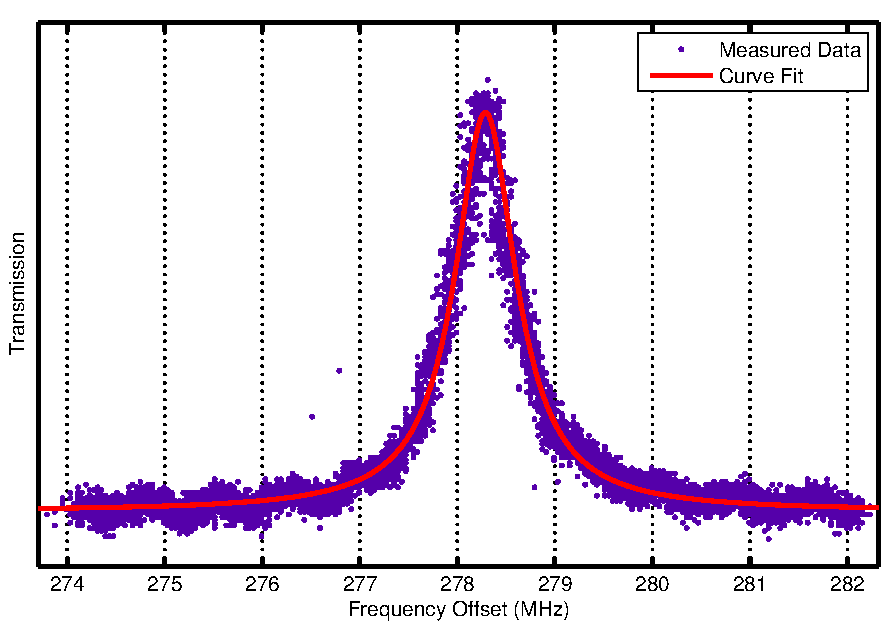
\includegraphics{figs-omc/FSRfit.pdf}
  \end{center}
  \caption{Measurement of the OMC FSR and cavity finesse. Fitted parameters give an FSR of $278.097 \pm 0.001$MHz and an finesse of $367\pm2$.}
  \label{fig:FSRfit}
\end{figure}

These data were taken with the OMC at room temperature. %NL%
It was discovered that the HOM spacing varied with the temperature of the thermal length actuator. %NL%
\com{Talk more about this? %NL%
it's own short section?}

\subsection{Higher order mode spacing}
Similarly, the higher order mode frequency shift is measured by varying the subcarrier frequency until the subcarrier is resonant on a higher order mode of the OMC. %NL%
Coupling of the subcarrier beam into the HOMs is enhanced if slight misalignments are introduced on the input beam. %NL%
The order of the mode is determined by the image recorded by the CCD in transmission.
\com{data here.}

\subsection{Cavity losses}
The intra-cavity loss of the OMC was infered by using 3 photodetectors. %NL%
One measuring a sample of the input light, one measuring the reflected light, and one measuring the transmitted light. %NL%
Care was taken to ensure that the three photodetectors were calibrated relative to each other.

\com{data here.}

\com{talk about degredation seen by squeezers}

\subsection{PZT actuator response}
The PZT length actuator of the OMC was calibrated using by using the PZT to sweep the cavity through both carrier and subcarrier resonances while recording the PZT voltage. %NL%
The frequency spacing of the carrier and subcarrier is used to calibrated the PZT length actuation coefficient.

\com{PZT sweep figure here.}

The frequency response of the PZT actuator was measured at the error signal of the cavity frequency locking loop while driving the OMC PZT. %NL%
The effects of the control loop have been removed from the data.

\com{TF here.}

\section{Opto-thermal-mechanical feedback issues in the OMC}

\com{At least include measurements by Tim and I, hopefully can hack a model to explain it.}

%%% Local Variables: 
%%% mode: latex
%%% TeX-master: "main"
%%% End: 
